\subsection{EntityHandle als virtuelles GameObject}

Mit der Einführung des ECS wird unter einem \texttt{GameObject} in \textit{helios} ein abstraktes Konzept einer Entität verstanden, die zur Laufzeit aktiv an den Spielmechaniken beteiligt ist.
Die Klasse \texttt{GameObject} ist dabei nicht mehr als konkrete Datenstruktur implementiert, sondern fungiert als virtuelle Abstraktion, die lediglich ein 8 Byte großes \texttt{EntityHandle} kapselt.
Von diesem Handle werden 4 Byte für die als \texttt{uint32\_t} typisierte \texttt{EntityId} verwendet, während die verbleibenden 4 Byte für eine gleich typisierte \texttt{VersionId} reserviert sind.
Diese \texttt{VersionId} repräsentiert einen Generationsindex, der die sichere Wiederverwendung von \texttt{EntityId}s ermöglicht.
Dies ist eine notwendige Voraussetzung, um die dichte Anordnung innerhalb der durch die \textit{Sparse Sets} realisierten Arrays zu ermöglichen.

\subsubsection{Generational Indexing als Identitätskonzept}

Das \texttt{EntityHandle} als zusammengesetzter Schlüssel folgt dem Konzept des \textit{Generational Indexing}~\cite{RCCK25}.\footnote{
    Datencontainer, die solche Daten speichern, werden auch als \textit{Slot Maps} bezeichnet~\cite{CppSlotMap}.
}.
Anschaulich lässt sich ein solches Handle mit einem Primärschlüssel in einem relationalen Datenbanksystem vergleichen, der auf die zugehörigen Datensätze verweist, ohne deren Inhalte selbst zu enthalten.
Die eindeutige Identifizierung eines solchen Objekts, welches im Kern eine lose Sammlung von Komponenten darstellt (anschaulich: Verteilt über verschiedene Tabellen) erfolgt zur Laufzeit ausschließlich über diesen zusammengesetzten Schlüssel.

\subsubsection{Gültigkeit, \textit{stale} Handles und Tombstones}

Die referenzierten Komponenten sind nur so lange gültig, wie der zusammengesetzte Schlüssel in der \texttt{EntityRegistry} als aktiv (\texttt{isValid()}) geführt wird.
Ein Handle gilt als ungültig - und ein Eintrag im \textit{Sparse Set} damit als \textit{stale} - sobald die \texttt{VersionId} des Handles (siehe Abbildung~\ref{fig:entityhandle}) nicht mehr mit der aktuell in der Registry hinterlegten Version für den entsprechenden Index übereinstimmt, der die \texttt{EntityId} repräsentiert.

Zur Markierung ungültiger Positionen in den \textit{Sparse Sets} werden sogenannte \textit{Tombstones} verwendet; dadurch lässt sich die Gültigkeitsprüfung effizient gestalten.\footnote{
    Ein \texttt{EntityTombstone} ist eine Konstante vom Typ \texttt{size\_t} und wird in \textit{helios} mit dem Wert \texttt{std::numeric\_limits<size\_t>::max()} initialisiert.
    Das Konzept ist auch in anderen Bereichen der Softwareentwicklung bekannt, etwa in Datenbanksystemen, in denen gelöschte Einträge zunächst markiert werden, um sie zu einem späteren Zeitpunkt physisch zu entfernen.~\cite{TombstoneApacheCassandra}
}

\begin{figure}[H]
    \centering
    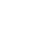
\includegraphics[width=0.8\columnwidth]{content/de/architektur/ecs/img/entityhandle}
    \caption{UML der Klasse \texttt{EntityHandle}. (Quelle: eigene Darstellung)}
    \label{fig:entityhandle}
\end{figure}

\subsubsection{Verwaltung durch \texttt{EntityRegistry} und \textit{Free List}}

Die Verwaltung und Neuerstellung von Handles wird durch die \texttt{EntityRegistry} auf Anfrage des \texttt{EntityManager}s realisiert.
Dabei werden innerhalb einer \textit{Free List} bereits gelöschte IDs verwaltet, deren Positionen in den \textit{Sparse Sets} durch einen \textit{Tombstone} repräsentiert werden.
Enthält die \textit{Free List} einen Eintrag, wird für den jeweiligen Index in der Registry die Versionsnummer inkrementiert und anschließend ein neues Handle bestehend aus Index und aktualisierter Versionsnummer zurückgegeben.
So können Indizes wiederverwendet werden, aber aufgrund der aktualisierten Versionsnummer dennoch von \textit{stale} Indizes unterschieden werden.
Sollte die \textit{Free List} keine Einträge beinhalten, wird der zugrunde liegende Vektor um einen neuen Eintrag erweitert und erhält die Versionsnummer $1$.

\vspace{5mm}
\begin{tcolorbox}[colback=black!5, colframe=black, title={Wertebereich von \texttt{EntityId}}]
    Bei einem Wertebereich von $2^{32}$ und unter der Annahme, dass theoretisch alle 16\,ms eine neue Version für eine spezifische \texttt{EntityId} erzeugt werden müsste, könnte ein entsprechendes Spiel etwa $2^{32} \cdot 0{,}016$ Sekunden lang betrieben werden, bevor ein Wertüberlauf eintritt.
    Dies entspricht einer Zeitspanne von knapp 795 Tagen.
    Damit ist ein ausreichender Puffer vorhanden, der weitgehend vernachlässigt werden kann, wenn \textit{Object Pooling} eingesetzt wird, um eine ständige Neuerzeugung von Objekten zur Laufzeit zu vermeiden.
    Ein Wechsel auf \texttt{uint64\_t} würde den theoretischen Zeitraum bis zu einem Überlauf auf etwa 9 Milliarden Jahre ausdehnen.
\end{tcolorbox}
\vspace{5mm}